\chapter{Método experimental e análise de resultados}
\label{chp:capitulo4}

Para avaliar o desempenho do aRPC foram executados vários casos de teste, todos eles implementados utilizando o aRPC e para efeitos de comparação, também implementados com o gRPC, sendo que tais testes são descritos na Seção \ref{sec:testes_propostos}. A partir desses testes foram coletadas uma série de métricas de interesse, explicitadas na Seção \ref{sec:metricas_interesse}. Os testes foram executados numa LAN fechada, entre dois computadores físicos, sendo um o cliente e outro o servidor, as características de \textit{hardware} e alguns detalhes de \textit{software} relativos a execução dos testes são levantados na Seção \ref{sec:infraestrutura_execucao}. Por fim, é feita uma análise dos dados obtidos em diversos cenários de execução, tal como a comparação de desempenho entre trafegar dados sem perda de pacotes ou com perda de pacotes e dentro e fora de estrutura de nuvem. Tais resultados são conferidos na Seção \ref{sec:resultados}.

\section{Casos de teste propostos}
\label{sec:testes_propostos}

Parte dos testes construídos foram baseados no trabalho de \cite{bagci_lightweight_2016} e outra parte foi desenvolvida como validação adicional. Neste sentido, os testes implementados baseados no artigo do HPRPC foram:

\begin{itemize}
	\item \textbf{Média}: Na referência essa operação, chamada de \textbf{Average}, recebe uma \textit{struct} contendo uma lista de \textbf{int32} e retorna a média dos números recebidos em \textbf{double}. Esse teste no artigo do HPRPC tem o propósito de avaliar o comportamento do \textit{framework} em requisições com características discrepantes de tamanho, onde a entrada é grande e a saída pequena.
	\item \textbf{Gerador de Números Aleatórios}: Na referência essa operação é chamada de \textbf{GetRandNums} e recebe um único número \textbf{int32} como entrada, que descreve uma quantidade. Em seguida é gerada uma lista de números pseudo aleatórios (\textbf{int32[]}) com tamanho equivalente à quantidade recebida. Esta operação foi usada para avaliação do HPRPC no cenário de requisições com características discrepantes de tamanho, onde a entrada é pequena e a saída grande.

	\item \textbf{Ecoar}: Na referência a operação é chamada de \textbf{SendRcvLargeData} e recebe uma lista de \textbf{int32} e retorna a mesma lista de \textbf{int32}. Este teste funciona como um \textit{echo server} e é utilizado para testes onde a entrada e a saída tem tamanhos equivalentes, avaliando o HPRPC em um cenário onde as requisições e respostas são igualmente grandes.
\end{itemize}

No trabalho sobre o HPRPC, os autores explicitam que foram feitas otimizações no serializador a fim de gerar ganhos no caso da transmissão de \textit{arrays} de tipos básicos, por esta razão, a maior parte dos testes propostos usam \textit{arrays} de \textbf{int32}, que justifica os bons resultados do \textit{framework}. Entretanto, tais testes são incompletos no sentido de comprovar a eficácia do HPRPC como um \textit{framework} RPC para uso no contexto mais geral de HPC. Por essa razão, a avaliação proposta pelo autores foi complementada neste trabalho com testes de velocidade e tamanho de serialização de requisições e respostas para todos os tipos básicos suportados pelo Colfer e o Protobuffers. 

Além disso, também foi efetuado um novo teste que recebe como argumento um \textit{array} de \textit{structs} que possuem todos os tipos suportados pelo Protobuffers e Colfer, este teste foi nomeado de \textbf{Todos os Tipos}. A justificativa para este novo teste é trazer para a avaliação do \textit{framework} de RPC informações que auxiliem na medição do desempenho em um caso de uso menos sintético. Outro ponto de melhoria foi a extensão dos testes para dados maiores, em um contexto de HPC faz sentido com que os dados transferidos ultrapassem a casa dos kilobytes, entretanto, os testes do HPRPC se limitam a quantidades de dados inferiores a dez mil elementos em \textbf{int32}, ou seja, igual ou menor que 40KB.


\section{Métricas de interesse}
\label{sec:metricas_interesse}

Em todos os testes foram coletados os tamanhos da requisição e da resposta, tempo serialização e desserialização da requisição e da resposta, tempo de execução do procedimento e tempo total. Usando esses dados é possível calcular o tempo de protocolo e transferência avaliando a seguinte equação:

\begin{equation}  
\label{eq:tempo_transmissao_protocolo}
    T_{TXPR}  =  T_{TOT} - T_{SERQ} - T_{DSRQ} - T_{SERE} - T_{DSRE} - T_{EX}
\end{equation}

Onde: 

\begin{eqnarray*} 
T_{TXPR} & = & tempo ~de ~transmiss\tilde{a}o ~e ~protocolo \\
T_{TOT}  & = & tempo ~total  \\
T_{SERQ} & = & tempo ~de ~serializa\textit{\c{c}}\tilde{a}o ~e ~requisi\textit{\c{c}}\tilde{a}o \\
T_{DSRQ} & = & tempo ~de  ~desserializa\textit{\c{c}}\tilde{a}o ~e ~requisi\text{\c{c}}\tilde{a}o  \\
T_{SERE} & = & tempo ~de ~serializa\textit{\c{c}}\tilde{a}o ~e ~resposta  \\
T_{DSRE} & = & tempo  ~de  ~desserializa\textit{\c{c}}\tilde{a}o ~e ~resposta  \\
T_{EX} & = &  tempo ~de ~execu\textit{\c{c}}\tilde{a}o  \\
\end{eqnarray*}
%%%%%%%%%%%%%%%%%%%
% Escolher um dos dois formatos...
%%%%%%%%%%%%%%%%%%%%%%

Também é possível calcular o tamanho total referente aos dados serializados comparativamente entre o aRPC e o gRPC através da razão entre os tamanhos em bytes de ambos. Além disso, foi avaliada a vazão da requisição a partir da razão entre o tempo completo de requisição desde seu inicio até sua resposta, menos o tempo de execução do procedimento e a quantidade de bytes trafegados na rede.  O tempo de execução absoluto foi calculado também usando razão dos tempos entre o aRPC e o gRPC. Todos os dados foram coletados para uma quantidade crescente de elementos nas \textit{structs} de requisição e resposta. Como o aRPC é um protocolo com intuito de ser usado no contexto de HPC, é importante que ele escale bem conforme a quantidade de dados aumente.

Foi efetuada uma avaliação de cada teste com 1, 2, 4, 8 e 16 \textit{threads}, entretanto, observou-se que a interface de rede Gigabit fica saturada a partir de duas \textit{threads}, momento em que o desempenho dos protocolos avaliados não apresenta mais divergências relevantes. Portanto os resultados apresentados contam com execuções utilizando apenas uma \textit{thread}.

Com relação às métricas de captura de tempo, foi utilizada a função \textbf{time.Now()} da biblioteca padrão da linguagem Go \cite{golang_time_2021}. De acordo com a documentação da biblioteca, esta função proporciona precisão de nanosegundos na medição do tempo. No caso específico deste trabalho, onde o sistema operacional utilizado foi o Linux, pode-se conferir que o Go faz um \textit{link} com a função \textbf{clock\_gettime} do sistema, conforme visto em \cite{golang_golanggo_2021}, a documentação para esta chamada de sistema no Linux pode ser conferida em \cite{linux_clock_getres2_2021}. Tendo em vista tais características, a função escolhida para medição de tempo apresenta acurácia necessária para os propósitos deste trabalho. Apesar da precisão de tempo para a função de captura ser em nanosegundos, as métricas foram avaliadas apenas em escalas de micro e milissegundos, de modo a evitar possíveis ruídos.

\section{Infraestrutura de execução}
\label{sec:infraestrutura_execucao}

As decisões relativas à infraestrutura de execução foram divididas em duas partes, \textit{hardware} e \textit{software}, cujas características são descritas na Seção \ref{sec:infraestrutura_execucao_hardware} e na Seção \ref{sec:infraestrutura_execucao_software}.

\subsection{Hardware}
\label{sec:infraestrutura_execucao_hardware}

Para avaliar o \textit{framework} foram executados testes em três ambientes, que são descritos adiante e têm como propósito dar às avaliações maior abrangência e detectar possíveis problemas associados aos ambientes de teste. Os ambientes testados foram:

\begin{alineas}
	\item Máquinas pessoais com rede Gigabit:
	\begin{subalineas}
		\item Processador do cliente: Intel Core i7-8700k @ 3.70GHz;
		\item Memória do cliente: 32GB DDR4;
		\item Processador do servidor: Intel Core i7-3770K @ 3.50GHz;
		\item Memória do servidor: 16GB DDR3; e
		\item Rede 1 Gigabit.
	\end{subalineas}
	\item Nuvem Microsoft Azure:
	\begin{incisos}
	    \item Máquina do tipo Standard F4s v2
		\item Processador: Intel Xeon Platinum 8272CL @ 2.60GHz;
		\item Memória RAM: 8GB DDR4; e
		\item Rede 10 Gigabits. 
	\end{incisos}
	\item Nuvem Google Cloud Platform:
	\begin{alineas}
		\item Processador Intel Xeon E5-2699 v3 @ 2.30GHz;
		\item Memória RAM: 6GB DDR4; e
		\item Rede 10 Gigabits.
	\end{alineas}
\end{alineas}

\subsection{Software}
\label{sec:infraestrutura_execucao_software}

Do ponto de vista de software, muitas melhorias e automações foram implementadas a fim de possibilitar testes maiores e mais complexos sem necessidade de intervenção humana. Os seguintes artefatos foram projetados: uma arquitetura de compilação; escalonadores de execução; exportação de métricas; e um \textit{script} de processamento para geração dos gráficos e extração das métricas. Primeiro as máquinas são preparadas com os arquivos do projeto, em seguida são compilados os executáveis de cada teste (cliente e servidor), então são configurados os escalonadores com o número de amostras por teste, intervalo de \textit{threads} a serem testados, quais testes a serem executados, e no caso do escalonador do cliente, também é configurado o endereço do servidor. 

Após configuração do escalonador do cliente e do servidor, os testes são executados em ordem de número de \textit{threads}, e amostras, e cada teste é executado exatamente o número especificado de amostras. O escalonador inicia o servidor correto e em seguida o cliente conecta, ao fim do teste, ambos os \textit{endpoints} salvam os dados capturados em arquivos \textbf{.json}. No \textbf{.json} do servidor são armazenados os tempos de execução dos procedimentos, enquanto no \textbf{.json} do cliente são escritos os demais dados. Ao fim dos testes, os arquivos são colocados em um google drive, que é acessado por um \textit{script} no Google Colab que faz processamento dos dados e extração das métricas relevantes e geração dos gráficos disponíveis neste trabalho.

Para que a serialização e as medições sejam comparáveis, foi necessário executar um grande número de amostras (por volta de duas mil por teste) onde em cada uma delas foi gerada de forma automática um valor pseudo aleatório para cada campo. Essa estratégia foi empregada, pois dependendo do tamanho do dado, tanto o Protobuffers quanto o Colfer, usam estratégias de serialização distintas e nesse sentido, não seria possível comparar os resultados de forma consistente entre os testes.

Outro ponto que vários autores não se atentam é para o fato que o gRPC não possui como parte obrigatória o TLS, e por essa razão para que a execução seja segura e as comparações façam sentido, foi necessário utilizar TLS sobre gRPC, que segue o mesmo paradigma que TLS sobre HTTP/2. No caso do protocolo QUIC, usado pelo aRPC, o uso de TLS é nativo e integrado, sendo assim, a comunicação é sempre encriptada e autenticada. Com isso, todos os testes utilizaram TLS tanto no aRPC quanto no gRPC, mesmo que no caso dos nossos testes não tenham sido trafegados dados sensíveis. Desta forma, a comparação entre os dois \textit{frameworks} de RPC é adequada.

Devido a quantidade de testes executados e o grande número de configurações necessárias, essa tarefa se mostrou desafiadora. Na configuração atual a quantidade de dados que deve ser trocada para garantir validade estatística somado a velocidade das interfaces de rede fez com que os testes tivessem longas durações. A ordem de grandeza da quantidade de execuções é na casa de $10^6$ chamadas de RPC, cada uma executando I/O (\textit{input}/\textit{output}) e variando-se a quantidade de elementos de 128 a 65536, que por sua vez variam de 4 a 2085 bytes. Estimamos, considerando que todos os testes rodam com 2000 amostras, que um teste pode chegar a transmitir entre 0,98 MiB e 273,29 GiB de dados.

\begin{figure}[ht]
    \centering
    \caption{Tempo de serialização}
    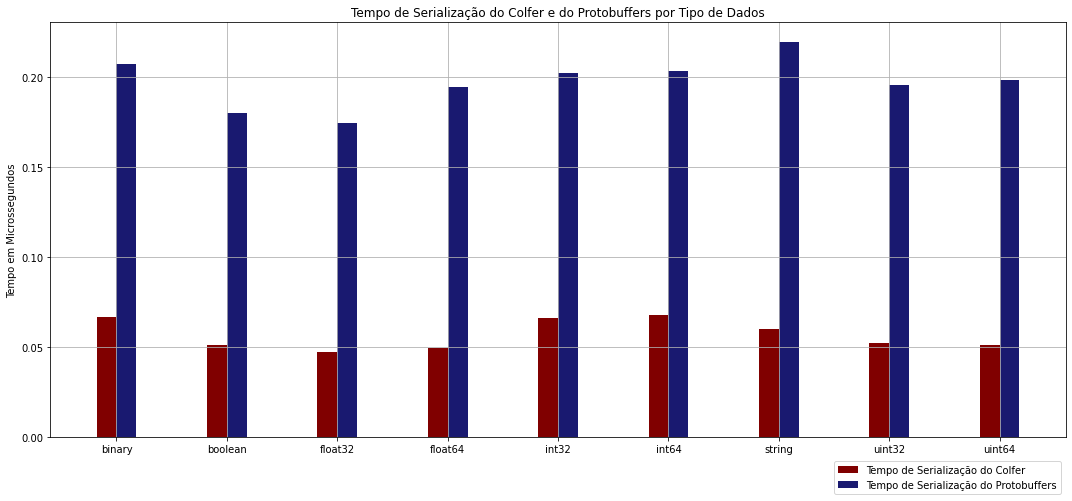
\includegraphics[width=\textwidth]{figuras/graficos/serializacao/tempo_serializacao.png} 
    \label{fig:tempo_serializacao}
\end{figure}

%%%%**** PAREI AQUI ****
\section{Resultados obtidos}
\label{sec:resultados}

De acordo com as métricas de interesse levantadas anteriormente, é possível dividir a análise dos resultados em três etapas. Uma etapa referente à serialização dos dados, outra etapa relacionada com o transporte dos dados pela rede e finalmente, uma etapa que engloba as características de desempenho do \textit{framework} de maneira mais completa.

\subsection{Serialização}

Para avaliar as métricas de serialização e desserialização, foram separados dois casos de uso distintos, realizando as operações para os tipos primitivos isoladamente e para os casos de teste mencionados anteriormente.

\subsubsection{Dados primitivos}

\begin{figure}[ht]
    \centering
    \caption{Tempo de desserialização}
    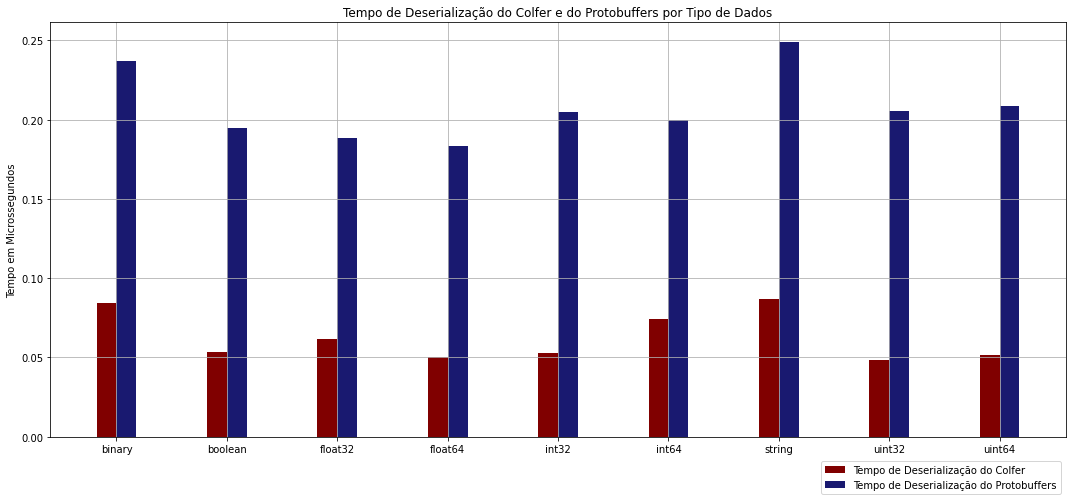
\includegraphics[width=\textwidth]{figuras/graficos/serializacao/tempo_deserializacao.png} 
    \label{fig:tempo_desserializacao}
\end{figure}

Foram realizadas medições do tempo de serialização, tempo de desserialização e tamanho dos dados serializados em ambos os serializadores, Colfer e Protobuffers. Todos os tipos primitivos compartilhados por ambos os serializadores foram testados. Estes são: \textbf{int32}, \textbf{int64}, \textbf{uint32}, \textbf{uint64}, \textbf{float32}, \textbf{float64}, \textbf{bool}, \textbf{binary} e \textbf{string}. Para a coleta desses dados, foram efetuados um milhão de testes por tipo de dado, os valores foram gerados aleatoriamente para cada execução e em seguida foi calculada a média dos tempos e tamanhos finais. Essa abordagem foi adotada porque os serializadores, tanto Protobuffers quanto Colfer, usam estratégias de serialização distintas para cada tipo e tamanho de dado para melhor otimizar o binário serializado. Dessa forma, com a abordagem aleatória e a média de uma grande quantidade de testes, é possível capturar a tendência para o caso de uso geral de cada tipo de dado em cada um dos serializadores. Essas três métricas podem ser conferidas nas Figuras \ref{fig:tempo_serializacao}, \ref{fig:tempo_desserializacao} e \ref{fig:tamanho_serializado}, respectivamente.

\begin{figure}[ht]
    \centering
    \caption{Tamanho dos dados serializados}
    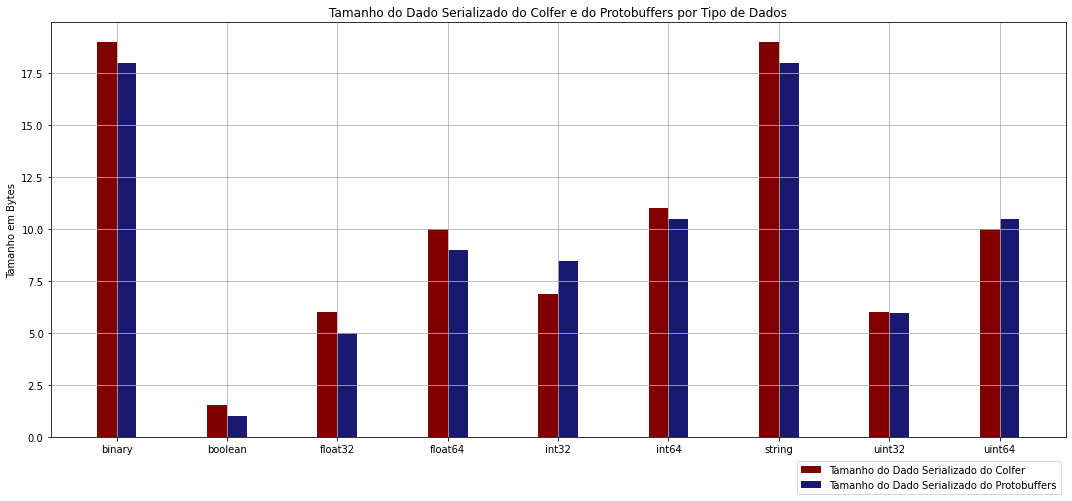
\includegraphics[width=\textwidth]{figuras/graficos/serializacao/tamanho_serializado.png} 
    \label{fig:tamanho_serializado}
\end{figure}

Conforme visto nas Figuras \ref{fig:tempo_serializacao} e \ref{fig:tempo_desserializacao}, é possível perceber que o Colfer consegue serializar os tipos primitivos de maneira mais rápida do que o Protobuffers, o ganho de \textit{speedup} pode ser conferido na Tabela \ref{tab:speedup_tipos_serializacao_desserializacao}.

%%%%%%%%%%%%%%%%%%%%%%%%%%%%%%%%%%%%%%%%%%%%%%%%%%%%%%%%%%%%%%%%%%%%%%%%%%%%%%%%%%%%%%%%%%%%%%%%%%%%%%%%%%%%%%%%
\begin{table}[H]
\centering
\caption{Speedups de serialização e desserialização obtidos para os tipos primitivos}
\label{tab:speedup_tipos_serializacao_desserializacao}
\begin{tabular}{llccc}
\hline
Tipos &  & \begin{tabular}[c]{@{}c@{}}Speedup \\ serialização\end{tabular} &  & \begin{tabular}[c]{@{}c@{}}Speedup \\ desserialização\end{tabular} \\ \hline
\textbf{int32}   &  & 3,0727 &  & 3,8864 \\
\textbf{int64}   &  & 3,0088 &  & 2,6963 \\
\textbf{uint32}  &  & 3,7620 &  & 4,2266 \\
\textbf{uint64}  &  & 3,9021 &  & 4,0461 \\
\textbf{float32} &  & 3,7297 &  & 3,0500 \\
\textbf{float64} &  & 3,9359 &  & 3,6593 \\
\textbf{binary}  &  & 3,1084 &  & 2,7994 \\
\textbf{bool}    &  & 3,5375 &  & 3,6591 \\
\textbf{string}  &  & 3,6759 &  & 2,8612 \\ 
\hline
\end{tabular}
\end{table}
%%%%%%%%%%%%%%%%%%%%%%%%%%%%%%%%%%%%%%%%%%%%%%%%%%%%%%%%%%%%%%%%%%%%%%%%%%%%%%%%%%%%%%%%%%%%%%%%%%%%%%%%%%%%%%%%

De acordo com a Figura \ref{fig:tamanho_serializado}, que apresenta o tamanho final dos dados serializados, é possível notar que o Protobuffers serializa os dados dos tipos \textbf{binary}, \textbf{boolean}, \textbf{float32}, \textbf{float64}, \textbf{int64} e \textbf{string} com uma quantidade menor de bytes, enquanto que os resultados são equivalentes para o caso \textbf{uint32} e que os dados de tipo \textbf{int32} e \textbf{uint64} são serializados pelo Colfer com tamanhos finais menores.

\subsubsection{Casos de teste}

Também foram avaliados o desempenho de serialização, com relação à razão entre o tamanho dos dados gerados pela serialização do aRPC e do gRPC, a partir dos dados relativos aos casos de teste propostos:
\textbf{Média}, \textbf{Gerador de Números Aleatórios}, \textbf{Ecoar} e \textbf{Todos os Tipos}. 
Cabe ressaltar que o teste \textbf{Todos os Tipos} recebe uma resposta vazia como resposta. 

\begin{figure}[ht]
    \centering
    \caption{Tamanho dos dados para o teste \textbf{Média}}
    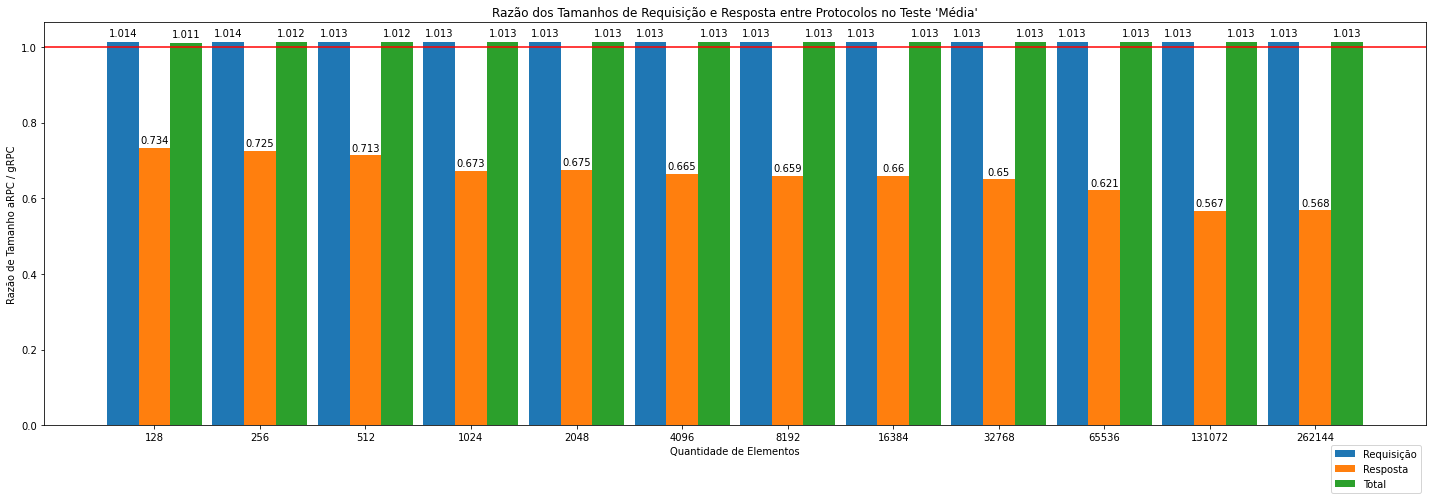
\includegraphics[width=\textwidth]{figuras/graficos/serializacao/razao_tamanho_average.png} 
    \label{fig:razao_tamanho_average}
\end{figure}

No teste \textbf{Média}, referente à Figura \ref{fig:razao_tamanho_average}, é possível observar que os tamanhos em bytes do aRPC transmitidos em cada procedimento (requisição + resposta) são de 1,1\% a 1,3\% maiores que o gRPC. Ou seja, o Colfer, apesar de muito mais rápido na serialização e desserialização, gera para este caso de testes dados ligeiramente maiores que o Protobuffers. 

Outra característica interessante que pode ser percebida na Figura \ref{fig:razao_tamanho_average} é que o tamanho da resposta do aRPC em relação ao gRPC tende a diminuir com o aumento do número de elementos presentes na requisição. Isso ocorre porque conforme a quantidade de elementos aumenta, fica mais provável que a média esteja próxima do centro do intervalo, que é o número zero. Nessa situação observa-se na Figura \ref{fig:tamanho_serializado} que o Colfer é mais eficiente que o Protobuffers na serialização de \textbf{int32}. Após uma análise, foi possível concluir que isso ocorre devido a uma ineficiência de serialização de valores negativos no Protobuffers.

Todos os valores negativos são serializados com 11 bytes no gRPC, independente do valor absoluto do número, enquanto que no aRPC os valores negativos são serializados usando cada vez menos bytes conforme o valor dos números negativos diminui. Como a divergência dos tamanhos nos números negativos entre os dois protocolos é mais acentuada próxima ao centro do intervalo, o número de elementos mais eficientemente codificados pelo aRPC aumenta em relação ao gRPC nesse campo proporcionalmente ao tamanho da resposta. Espera-se que esse comportamento se estabilize com uma maior quantidade de elementos.

\begin{figure}[ht]
    \centering
    \caption{Perfil de execução para o teste \textbf{Média}}
    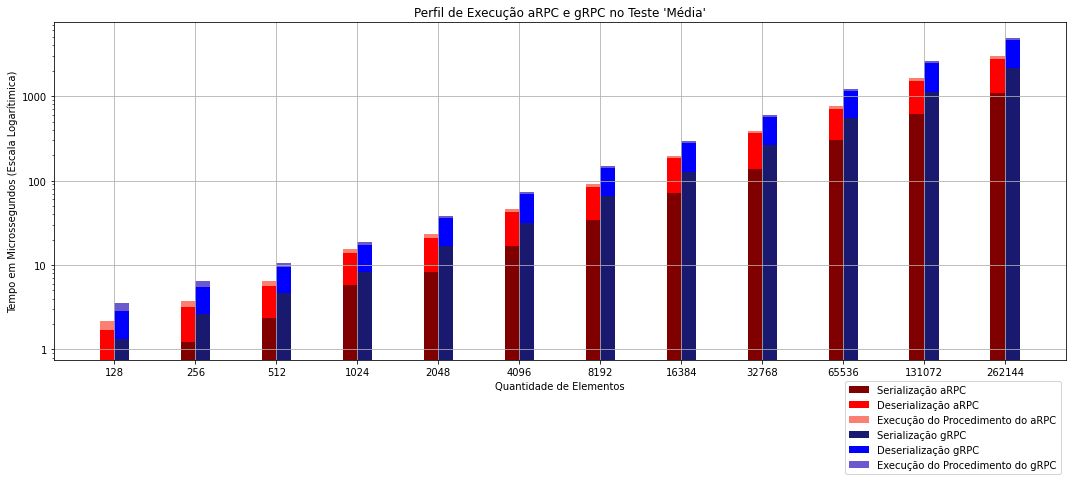
\includegraphics[width=\textwidth]{figuras/graficos/serializacao/perfil_execucao_average.png} 
    \label{fig:perfil_execucao_average}
\end{figure}

É interessante observar que, apesar do teste \textbf{Média} no aRPC ter gerado dados levemente maiores que o gRPC, o ganho referente aos tempos de serialização e desserialização são significativos, como pode ser visto na Figura \ref{fig:perfil_execucao_average}. O menor ganho, nesse grupo de dados, é referente à quantidade de 512 elementos que teve \textit{speedup} de 1,4756, já o maior é referente ao caso com 128 elementos, que teve \textit{speedup} de 2,8698. Dessa forma, os ganhos em tempo de processamento na serialização ajudam a compensar a sobrecarga do envio de mais bytes pela interface de rede.


Quanto ao caso de teste \textbf{Gerador de Números Aleatórios}, na Figura \ref{fig:razao_tamanho_getrandomnumbers}, é interessante notar que o tempo total é dominado pela resposta, em contrapartida ao caso de teste anterior (\textbf{Média}) no qual a relevância maior foi do tempo de requisição. Quanto ao tamanho das requisições serializadas serem maiores no Colfer do que no Protobuffers, isso se dá pelo fato dos números inteiros positivos serem codificados de maneira mais otimizada no Protobuffers. Cabe ressaltar que os dados presentes na resposta também são todos números positivos, caso contrário o resultado seria mais favorável ao Colfer, tendo em vista que o mesmo otimiza melhor o tamanho de números negativos.

\begin{figure}[ht]
    \centering
    \caption{Tamanho dos dados para o teste \textbf{Gerador de Números Aleatórios}}
    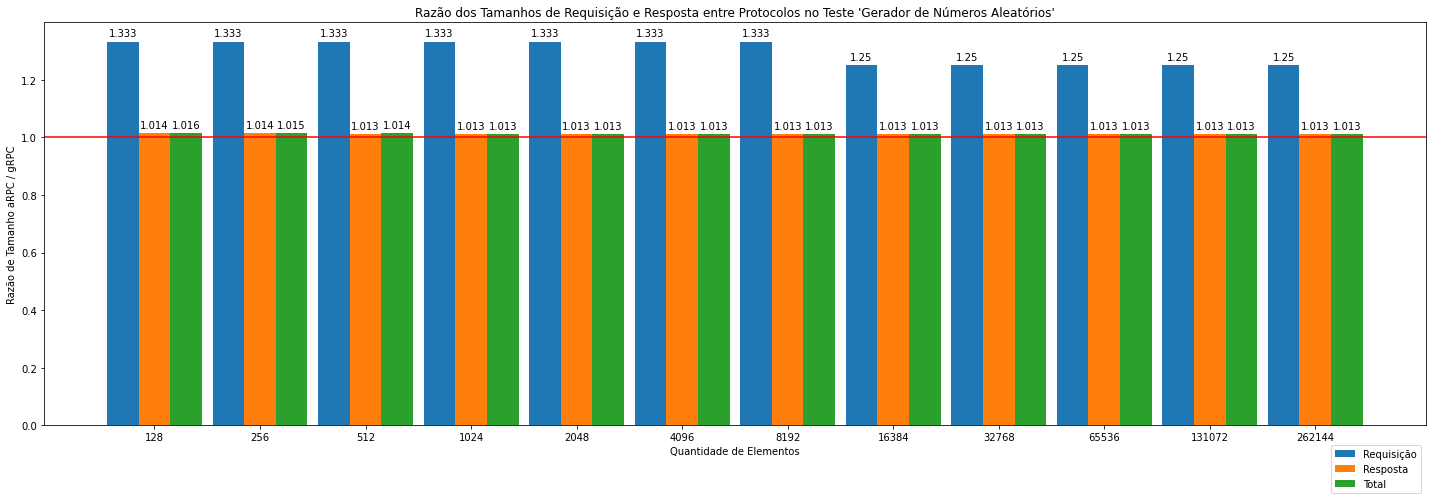
\includegraphics[width=\textwidth]{figuras/graficos/serializacao/razao_tamanho_getrandomnumbers.png} 
    \label{fig:razao_tamanho_getrandomnumbers}
\end{figure}

Na Figura \ref{fig:perfil_execucao_getrandomnumbers} é possível observar que no teste \textbf{Gerador de Números Aleatórios} o Colfer é mais eficiente para todas as quantidades de dados testadas, tendo \textit{speedups} nos tempos de execução variando de 1,1906 para 4096 elementos a 2,2543 para 128 elementos. Como justificado anteriormente, esse ganho ajuda a compensar a leve diferença de tamanho nos dados transmitidos. Além disso, é relevante ressaltar que o tempo de execução deste teste é maior que todos os outros e a quantidade de recursos consumidos é significativamente maior para a geração dos números aleatórios. Este fato é relevante para os resultados comparativos do tempo de execução do aRPC contra o gRPC neste teste.

\begin{figure}[H]
    \centering
    \caption{Perfil de execução para o teste \textbf{Gerador de Números Aleatórios}}
    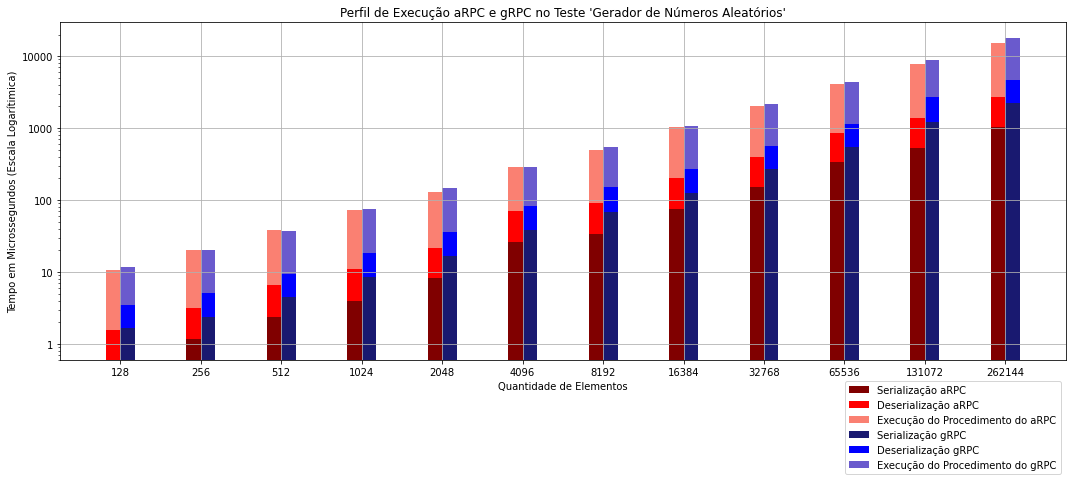
\includegraphics[width=\textwidth]{figuras/graficos/serializacao/perfil_execucao_getrandomnumbers.png} 
    \label{fig:perfil_execucao_getrandomnumbers}
\end{figure}

\begin{figure}[ht]
    \centering
    \caption{Tamanho dos dados para o teste \textbf{Ecoar}}
    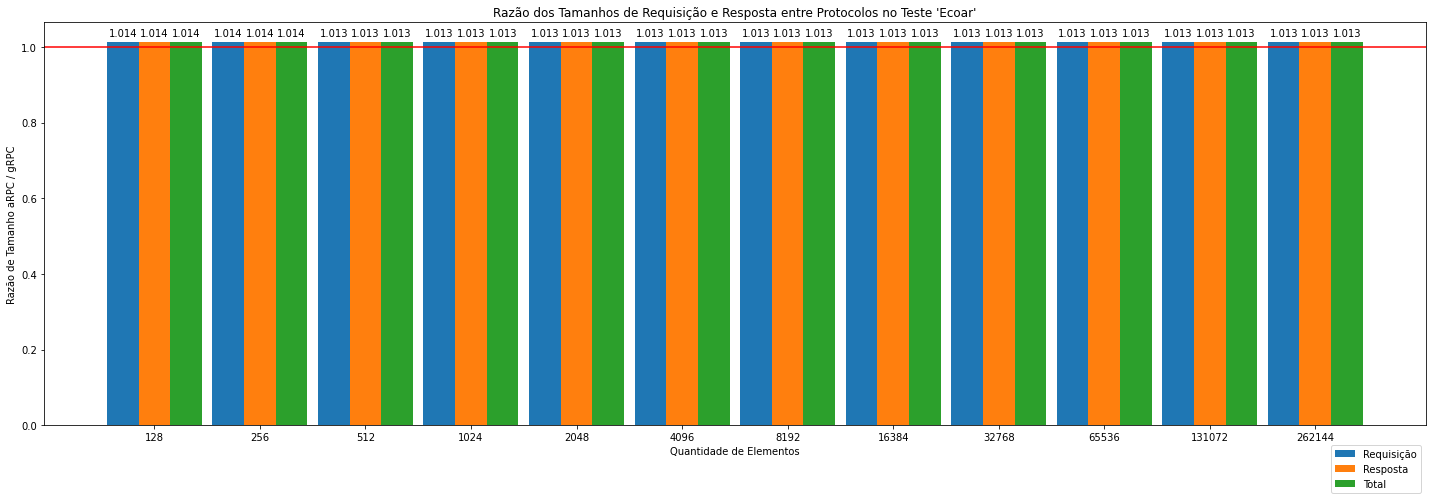
\includegraphics[width=\textwidth]{figuras/graficos/serializacao/razao_tamanho_largedata.png} 
    \label{fig:razao_tamanho_largedata}
\end{figure}

Nas Figuras \ref{fig:razao_tamanho_largedata} e \ref{fig:perfil_execucao_largedata} podem ser vista as análises de tamanhos e de tempos para o teste \textbf{Ecoar}. Neste teste o Colfer gerou dados 1,3\% a 1,4\% maiores que o Protobuffers, entretanto, com \textit{speedups} variando de 1,4730 para 1024 elementos à 1,9424 para 256 elementos.

\begin{figure}[ht]
    \centering
    \caption{Perfil de execução para o teste \textbf{Ecoar}}
    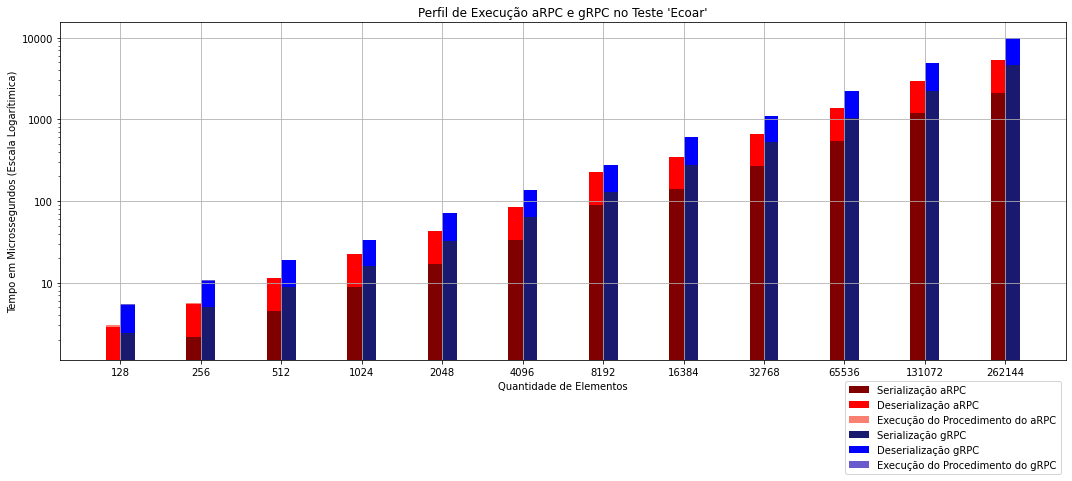
\includegraphics[width=\textwidth]{figuras/graficos/serializacao/perfil_execucao_largedata.png} 
    \label{fig:perfil_execucao_largedata}
\end{figure}

Na Figura \ref{fig:razao_tamanho_alltypes} é possível observar o primeiro caso onde o serializador do Colfer gerou dados menores que o Protobuffers para requisição, resposta e o total, para todas as quantidades de elementos testadas. Esse caso de teste foi desenvolvido a fim de averiguar os serializadores e protocolos em estruturas de dados heterogêneas, com o proposito de torná-lo mais representativo dos casos de uso reais. Nesse sentido, quando uma estrutura desse tipo é utilizada, o Colfer não somente mantém os \textit{speedups} altos em relação ao Protobuffers, nos tempos de serialização e desserialização, mas ainda gera um dado serializado em média 0,4\% menor, o que resulta em ganhos expressivos no tempo de execução do aRPC, que serão melhor detalhados à frente. Nesses testes é possível ver, através de análises da Figura \ref{fig:perfil_execucao_alltypes}, que os \textit{speedups} variam de 1,4756 para 512 elementos a 2,8698 para 128 elementos.

\begin{figure}[ht]
    \centering
    \caption{Tamanho dos dados para o teste \textbf{Todos os Tipos}}
    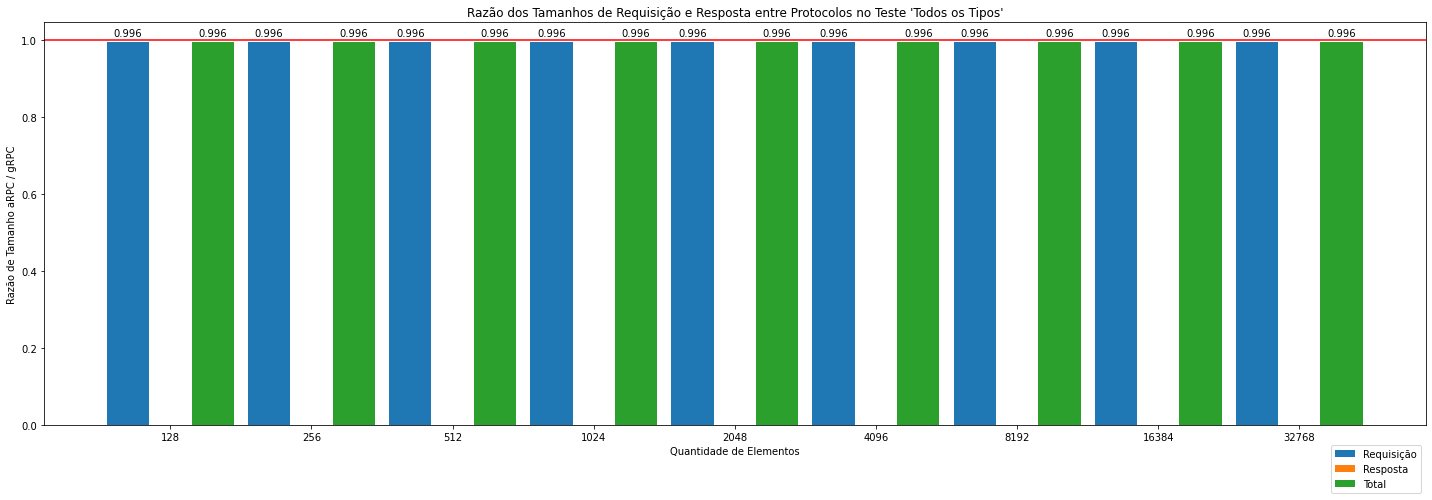
\includegraphics[width=\textwidth]{figuras/graficos/serializacao/razao_tamanho_alltypes.png} 
    \label{fig:razao_tamanho_alltypes}
\end{figure}

\begin{figure}[ht]
    \centering
    \caption{Perfil de execução para o teste \textbf{Todos os Tipos}}
    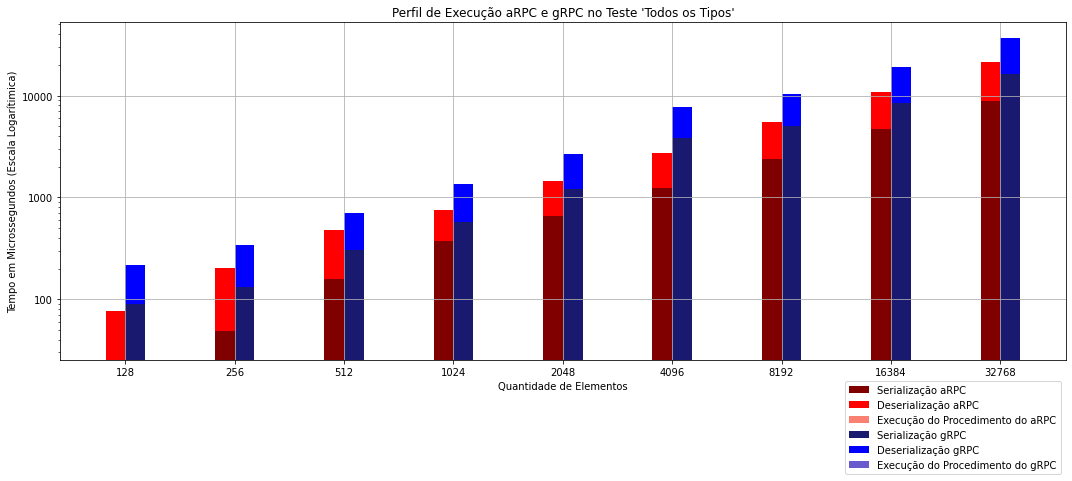
\includegraphics[width=\textwidth]{figuras/graficos/serializacao/perfil_execucao_alltypes.png} 
    \label{fig:perfil_execucao_alltypes}
\end{figure}

Através dessas análises, pode-se observar que o Colfer como serializador é consistente em relação ao \textit{speedup} de serialização e desserialização perante o Protobuffers, com valores entre 1,4730 e 2,8698. Outro fator relevante é que com o crescimento exponencial da quantidade de dados, o crescimento do tempo de execução também é exponencial. Indicando que o crescimento do tempo de serialização e desserialização é linear de acordo com o tamanho da entrada.

Nos testes onde o Colfer teve um tamanho de dados superior ao Protobuffers, esta sobrecarga nos tamanhos foi de 1,1\% a 1,6\%, enquanto que no caso de teste \textbf{Todos os Tipos} a redução de tamanho foi de 0,4\% em relação ao Protobuffers, ressaltando que este teste é mais próximo dos casos de uso reais. Logo, o \textit{speedup} de serialização e desserialização e eventuais ganhos no protocolo de transporte devem compensar esta sobrecarga para que o aRPC tenha desempenho melhor que o gRPC.

\begin{figure}[!ht]
    \centering
    \caption{Vazão do aRPC e do gRPC para o caso de teste \textbf{Todos os Tipos}}
    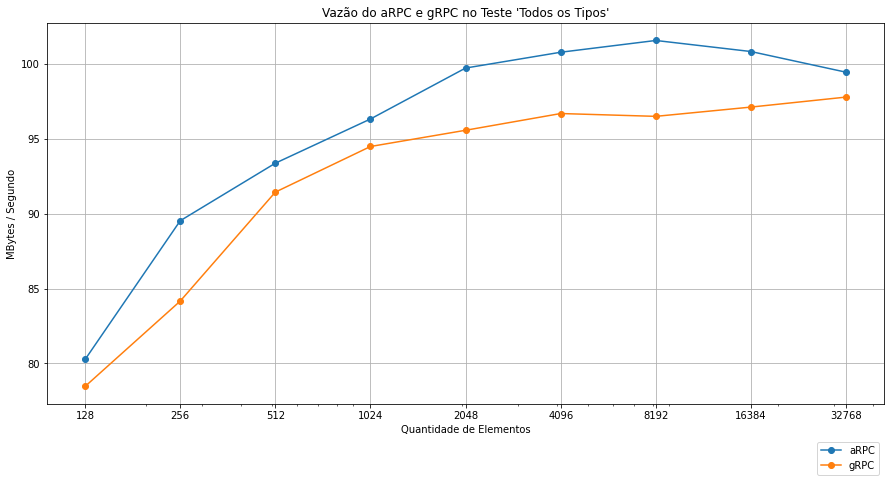
\includegraphics[width=\textwidth]{figuras/transporte/vazao_alltypes.png} 
    \label{fig:vazao_alltypes}
\end{figure}

\subsection{Transporte}

Nesta seção foram feitos os testes relacionados ao transporte dos dados em cenários com redes diferentes. Os ambientes foram: conjunto de máquinas pessoais numa LAN fechada, com rede 1 Gigabit e nuvens Microsoft Azure e Google Cloud Platform, ambas com rede de 10 Gigabits

\subsubsection{Máquinas pessoais}
\label{subsubsection:maquinas_pessoais}

Nas Figuras \ref{fig:vazao_alltypes}, \ref{fig:vazao_average}, \ref{fig:vazao_getrandomnumbers} e \ref{fig:vazao_largedata}, respectivamente para os casos de teste \textbf{Todos os Tipos}, \textbf{Média}, \textbf{Gerador de Números Aleatórios} e \textbf{Ecoar}, é possível se conferir que, devido aos dados mais heterogêneos, o aRPC se distancia do gRPC desde o início, até saturar a interface de rede. Enquanto nos demais testes, por tratarem apenas de dados do tipo \textbf{int32} o gRPC começa com vantagem, porém, conforme o número de elementos aumenta, o aRPC tende a superá-lo.

\begin{figure}[ht]
    \centering
    \caption{Vazão do aRPC e do gRPC para o caso de teste \textbf{Média}}
    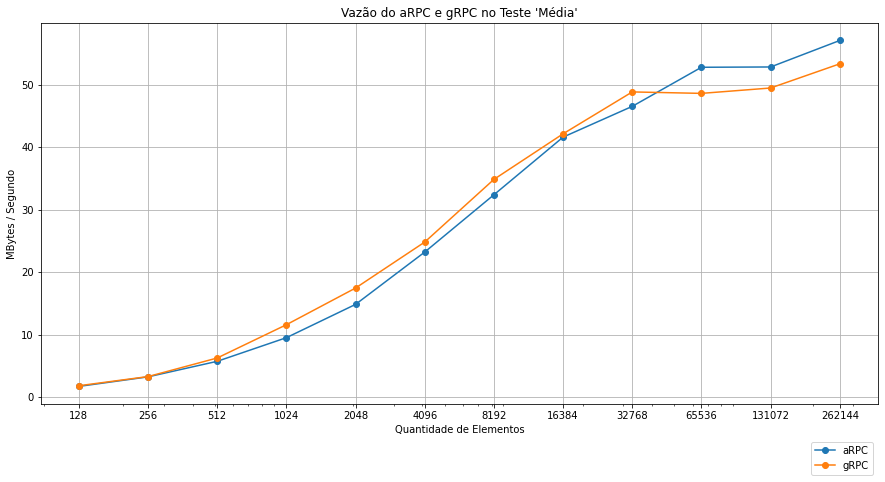
\includegraphics[width=\textwidth]{figuras/transporte/vazao_average.png} 
    \label{fig:vazao_average}
\end{figure}

\begin{figure}[ht]
    \centering
    \caption{Vazão do aRPC e do gRPC para o caso de teste \textbf{Gerador de Números Aleatórios}}
    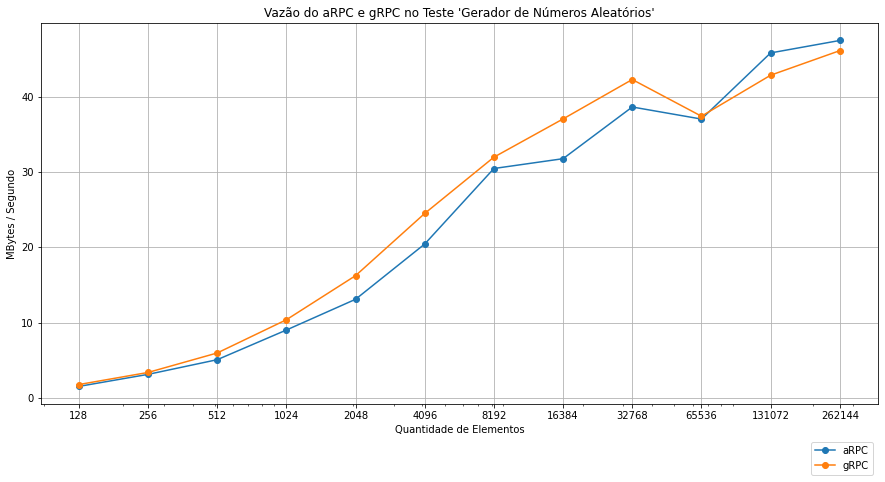
\includegraphics[width=\textwidth]{figuras/transporte/vazao_getrandomnumbers.png} 
    \label{fig:vazao_getrandomnumbers}
\end{figure}

\begin{figure}[ht!]
    \centering
    \caption{Vazão do aRPC e do gRPC para o caso de teste \textbf{Ecoar}}
    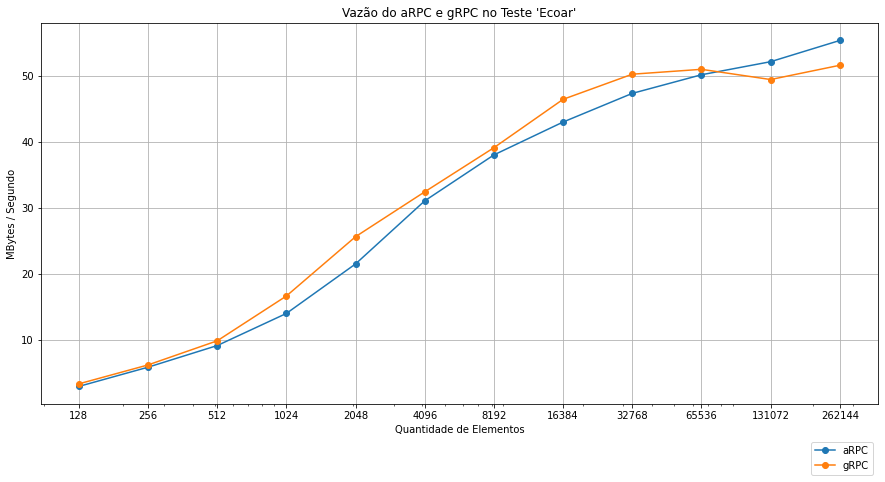
\includegraphics[width=\textwidth]{figuras/transporte/vazao_largedata.png} 
    \label{fig:vazao_largedata}
\end{figure}

Um teste foi executado simulando perda de pacotes na rede somente no ambiente de máquinas pessoais, devido ao maior controle sobre os parâmetros da rede. Para simular a perda de pacotes, foi executado o comando \textbf{sudo tc qdisc add dev enp0s31f6 root netem loss 5\%}, utilizando o módulo do kernel \textbf{sch\_netem}, conforme \cite{cardwell_networkingnetem_2021}. Esta perda de 5\% dos pacotes pode ser verificada utilizando o programa \textbf{ping}, conforme pode ser conferido nas Figuras \ref{fig:client_to_server} e \ref{fig:server_to_client}.

\begin{figure}[ht]
    \centering
    \caption{Resultados do comando \textbf{ping} do cliente para o servidor}
    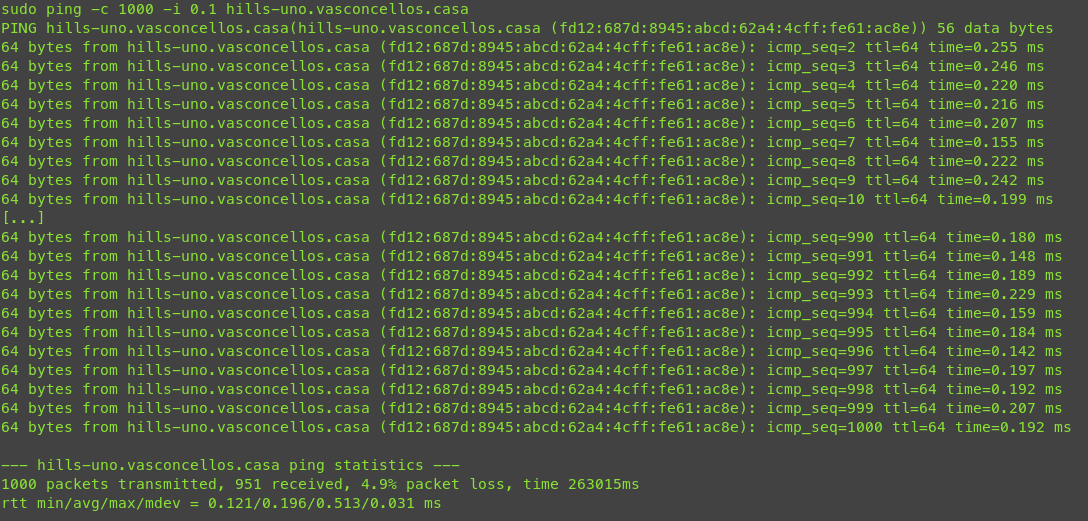
\includegraphics[width=0.9\textwidth]{figuras/transporte/client_to_server.png} 
    \label{fig:client_to_server}
\end{figure}

\begin{figure}[ht]
    \centering
    \caption{Resultados do comando \textbf{ping} do servidor para o cliente}
    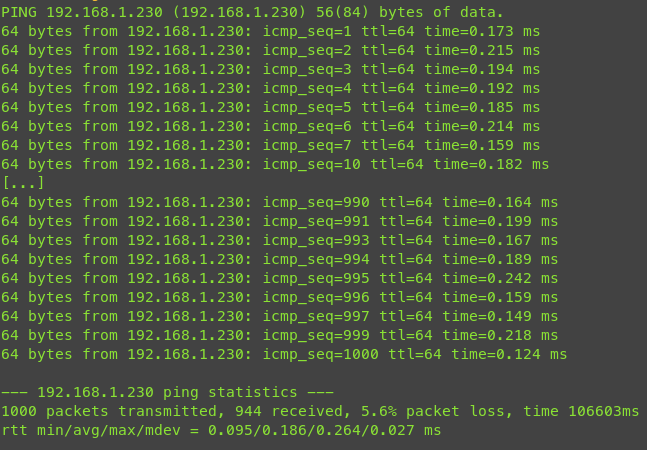
\includegraphics[width=0.6\textwidth]{figuras/transporte/server_to_client.png} 
    \label{fig:server_to_client}
\end{figure}

\begin{figure}[!ht]
    \centering
    \caption{Comparação entre aRPC e gRPC em cenários com e sem perda de pacotes}
    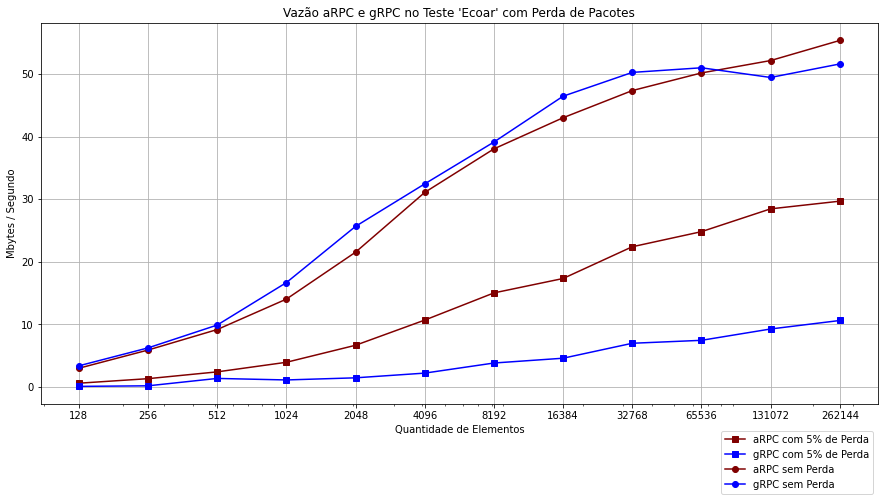
\includegraphics[width=\textwidth]{figuras/transporte/arpc_grpc_lossy.png} 
    \label{fig:arpc_grpc_lossy}
\end{figure}

Na Figura \ref{fig:arpc_grpc_lossy} é possível conferir os resultados encontrados para o aRPC e gRPC, de maneira comparativa, entre os cenários com perda de pacotes e sem perda de pacotes. Nela pode ser observado, que num cenário com maior perda de pacotes, as características do QUIC se destacam mais, tal como a prevenção ao problema de \textit{Head-of-Line Blocking}, tendo em vista que mesmo para uma quantidade pequena de dados a vazão do aRPC imediatamente se distancia da vazão do gRPC. Foi utilizado o caso de teste \textbf{Ecoar} pois ele utiliza o mesmo dado na requisição e na resposta.

\subsubsection{Microsoft Azure}

Neste ambiente, apesar da rede ser de 10 Gigabits, identificou-se que a transmissão de dados utilizando o QUIC tinha um desempenho comparativamente inferior ao TCP em relação àquele apresentado no ambiente das máquinas pessoais. Por isso, uma investigação foi realizada, utilizando o programa \textbf{iperf3}, para verificar o desempenho de transmissão entre as máquinas. O programa foi executado com tempo de teste de 300 segundos e tamanho do pacote UDP padrão, de 1460 bytes. Nos resultados foi averiguado que, enquanto a taxa de transmissão para o protocolos TCP estavam dentro dos valores esperados. A taxa de transmissão do UDP estavam sendo limitada, possivelmente devido a mitigações descritas na Seção \ref{subsec:udp}. Os resultados do \textbf{iperf3} podem ser conferidos nas Figuras \ref{fig:iperf_client_azure} e \ref{fig:iperf_server_azure}.

\begin{figure}[ht]
    \centering
    \caption{Resultados do \textbf{iperf3} executado no cliente na Microsoft Azure}
    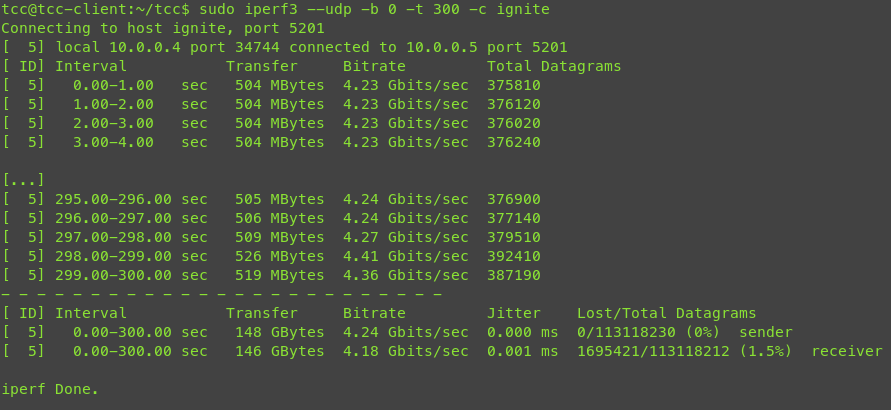
\includegraphics[width=0.8\textwidth]{figuras/transporte/iperf_client_azure.png} 
    \label{fig:iperf_client_azure}
\end{figure}

\begin{figure}[!ht]
    \centering
    \caption{Resultados do \textbf{iperf3} executado no servidor na Microsoft Azure}
    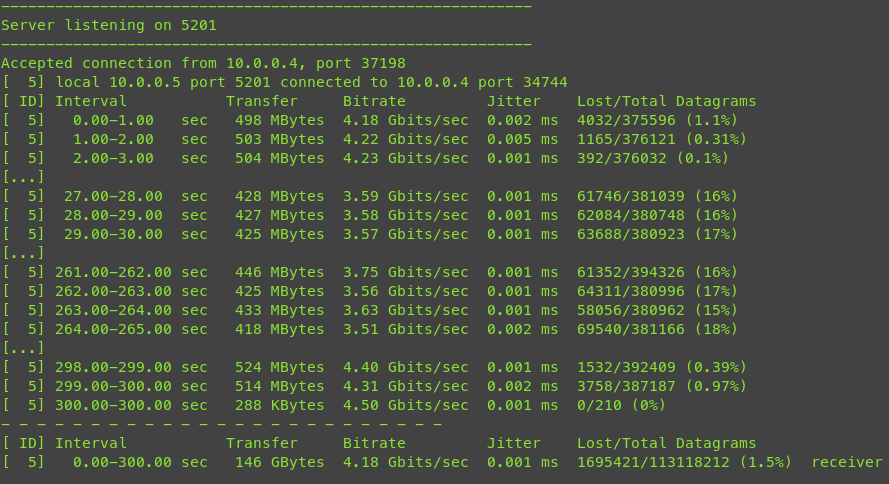
\includegraphics[width=0.8\textwidth]{figuras/transporte/iperf_server_azure.png} 
    \label{fig:iperf_server_azure}
\end{figure}

\subsubsection{Google Cloud Platform}

Assim como ocorreu no ambiente Microsoft Azure, foram observados limites aos protocolo UDP, que afetaram os resultados obtidos pelo aRPC. Portanto a mesma estratégia de análise com o \textbf{iperf3} foi empregada, que pode ser conferida nas Figuras \ref{fig:iperf_client_gcp} e \ref{fig:iperf_server_gcp}, justificando assim o desempenho encontrado.

\begin{figure}[ht]
    \centering
    \caption{Resultados do \textbf{iperf3} executado no cliente na Google Cloud Platform}
    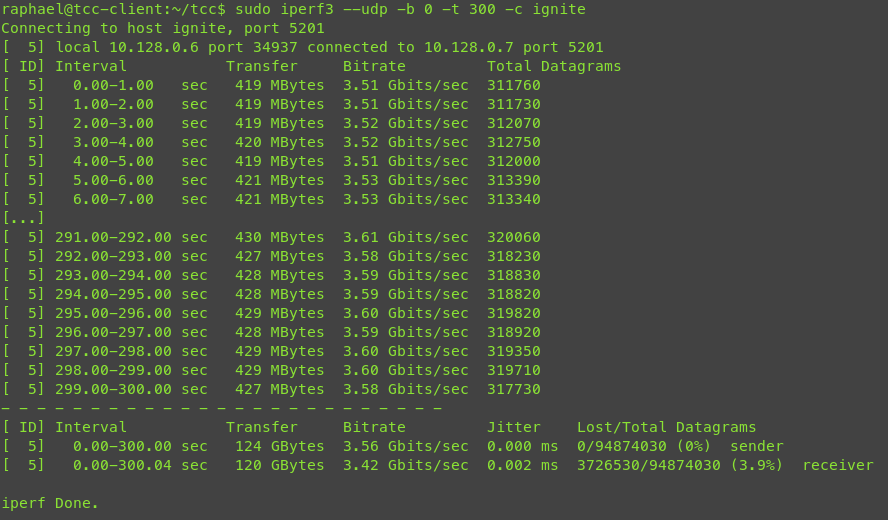
\includegraphics[width=0.8\textwidth]{figuras/transporte/iperf_client_gcp.png} 
    \label{fig:iperf_client_gcp}
\end{figure}

\begin{figure}[!ht]
    \centering
    \caption{Resultados do \textbf{iperf3} executado no servidor na Google Cloud Platform}
    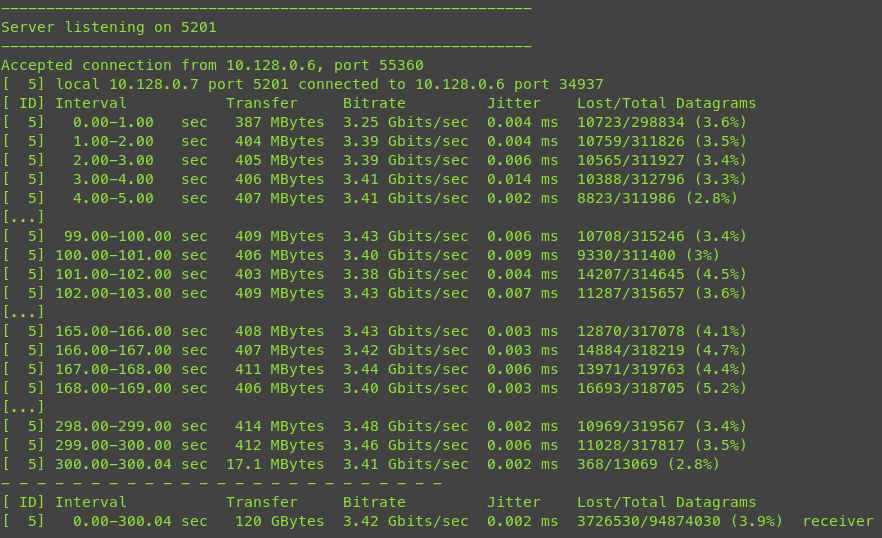
\includegraphics[width=0.8\textwidth]{figuras/transporte/iperf_server_gcp.png} 
    \label{fig:iperf_server_gcp}
\end{figure}

\begin{figure}[ht]
    \centering
    \caption{Razão entre as vazões do aRPC e do gRPC, entre os três ambientes}
    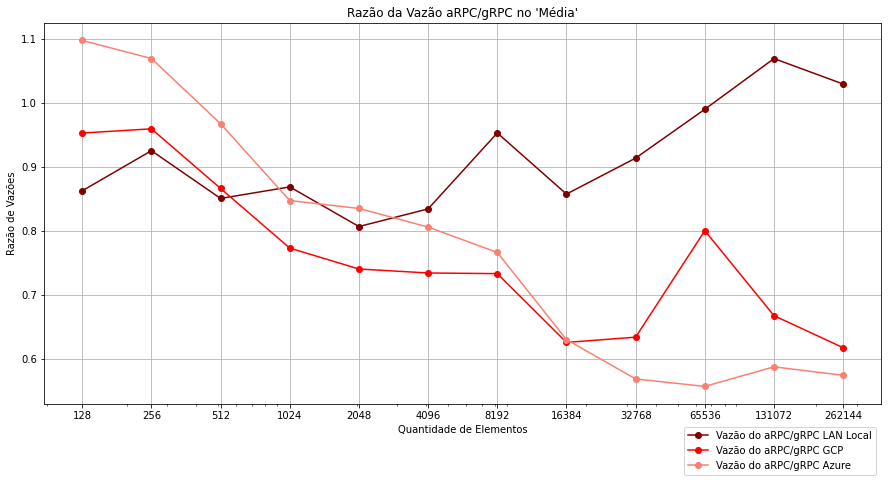
\includegraphics[width=\textwidth]{figuras/transporte/comparação_lan_azure_gcp.png} 
    \label{fig:comparação_lan_azure_gcp}
\end{figure}

\subsubsection{Comparação entre ambientes}

Devido aos estrangulamentos nas transmissões utilizando UDP nos ambientes de nuvem, foi feita uma comparação da evolução de escalabilidade entre os três ambientes, conforme visto na Figura \ref{fig:comparação_lan_azure_gcp}. Nela é possível averiguar que a razão entre as vazões cai conforme a quantidade de elementos aumenta, isso ocorre pois nos ambientes de nuvem existem configurações de sistema limitando a vazão do UDP, \ref{subsec:udp}. Devido a essa prática, o aRPC não é adequado a esses ambientes pois apesar de possuírem maior largura de banda, o protocolo acaba tendo seu desempenho limitado. É importante ressaltar que com a crescente adoção do QUIC, essas limitações devem ser removidas ou modificadas \cite{rossow2014amplification}, como justificado na Sessão \ref{subsec:quic}.

\subsection{\textit{Framework}}

A proposta do aRPC é ser um \textit{framework} simples para HPC que mantenha as características da linguagem e efetue chamadas de procedimentos remotos de forma transparente. Neste sentido, é importante que o \textit{framework} tenha desempennho melhor que o gRPC para grandes quantidades de elementos e em contextos de dados mais heterogêneos.

\begin{figure}[ht]
    \centering
    \caption{Tempo de execução do HPRPC e do gRPC}
    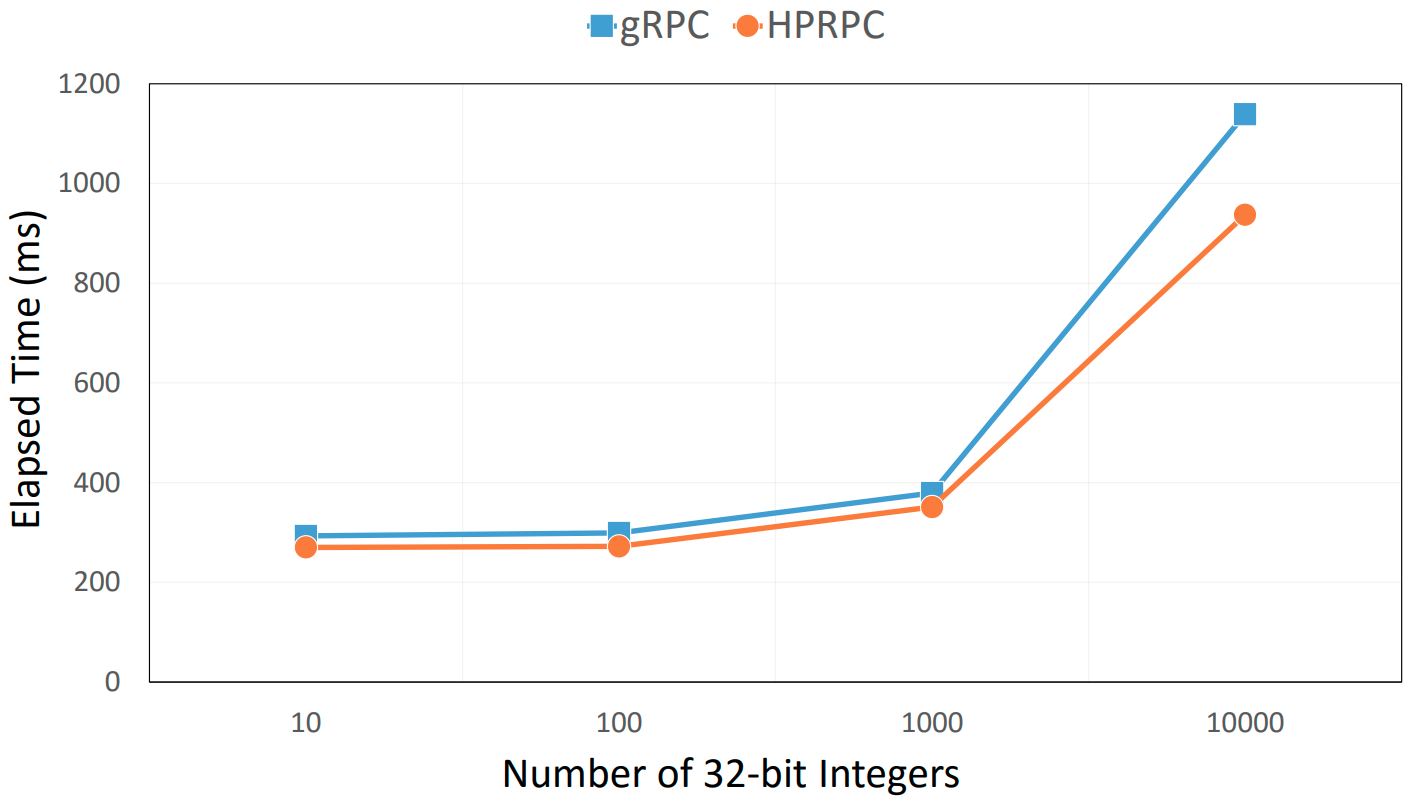
\includegraphics[width=0.7\textwidth]{figuras/framework/hprpc_time_measure.png}
    \label{fig:hprpc_time_measure}
    \legend{Fonte: \cite{bagci_lightweight_2016}}
\end{figure}

\begin{figure}[ht]
    \centering
    \caption{Tempo de execução do aRPC e do gRPC (Foco em $x \in [0;1000]$)}
    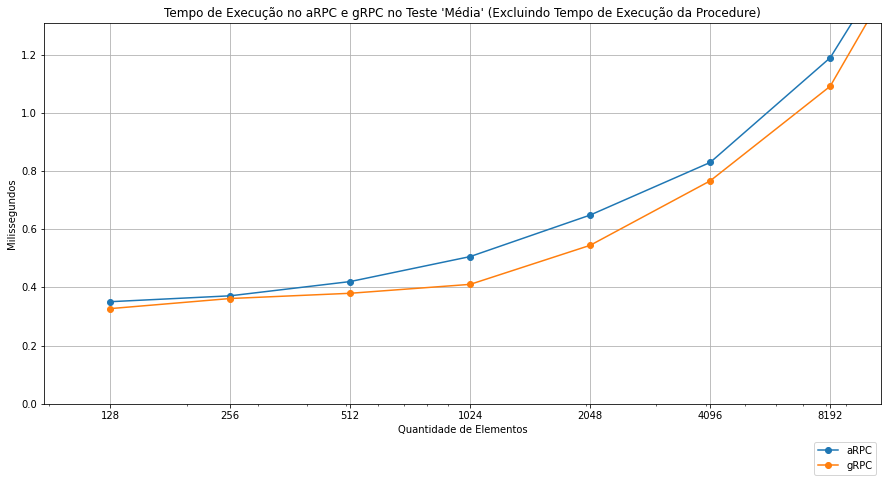
\includegraphics[width=\textwidth]{figuras/framework/tempo_execucao_abs_zoom_average.png}
    \label{fig:tempo_execucao_abs_zoom_average}
\end{figure}

No artigo do HPRPC o autor disponibiliza gráficos de tempo de execução, foram feitas as mesmas medições no gRPC e no aRPC para fins de comparação. Na Figura \ref{fig:hprpc_time_measure} é possível observar os dados coletados pelos autores do HPRPC. Na medição realizada nesse trabalho foi observada uma divergência em relação à unidade dos dados apresentados pelos autores no eixo Y. No artigo não é informada a largura de banda da rede e nem o \textit{hardware} utilizado, entretanto, para que 128 elementos \textbf{int32} e sua resposta \textbf{float64} sejam transferidos são necessários em torno de 520 bytes. 

Na Figura \ref{fig:hprpc_time_measure} o tempo de execução foi cerca de 300ms tanto para HPRPC e gRPC. Entretanto, esses valores apontam para uma vazão de 1,3 KB/s e esse é um valor suspeito, uma vez que seria necessário um hardware muito antigo para que o gRPC tenha esse tempo de execução. Como pode ser visto na Figura \ref{fig:tempo_execucao_abs_zoom_average} o gRPC tem um tempo de transferência por volta de 0,3 ms para essa ordem de grandeza de dados. Isso levanta possíveis indícios de que as medições estão em microssegundos e não em milissegundos como indicado. Sendo assim, não foi possível realizar os testes comparativos planejados com o HRPC.

\begin{figure}[!ht]
    \centering
    \caption{Razão do Tempo de execução do aRPC e do gRPC para o caso de teste \textbf{Ecoar}}
    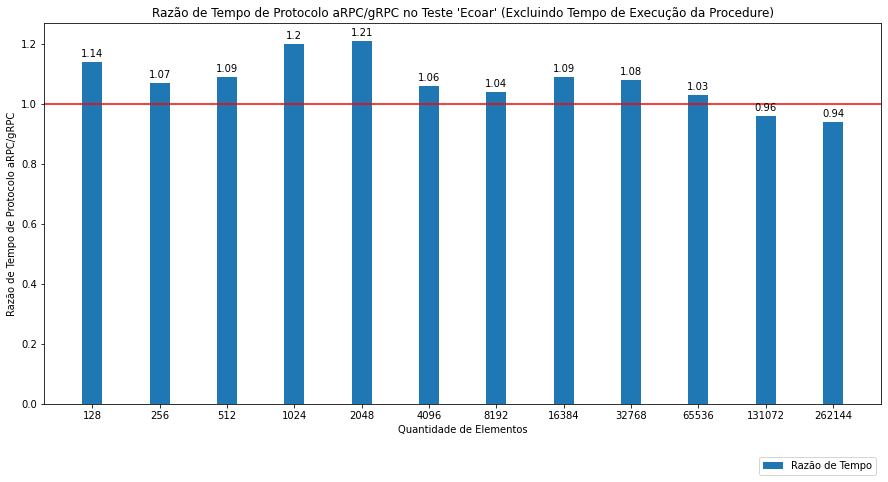
\includegraphics[width=\textwidth]{figuras/framework/razao_tempo_execucao_largedata.png}
    \label{fig:razao_tempo_execucao_largedata}
\end{figure}

\begin{figure}[!ht]
    \centering
    \caption{Razão do Tempo de execução do aRPC e do gRPC para o caso de teste \textbf{Gerador de NúmerosAleatórios}}
    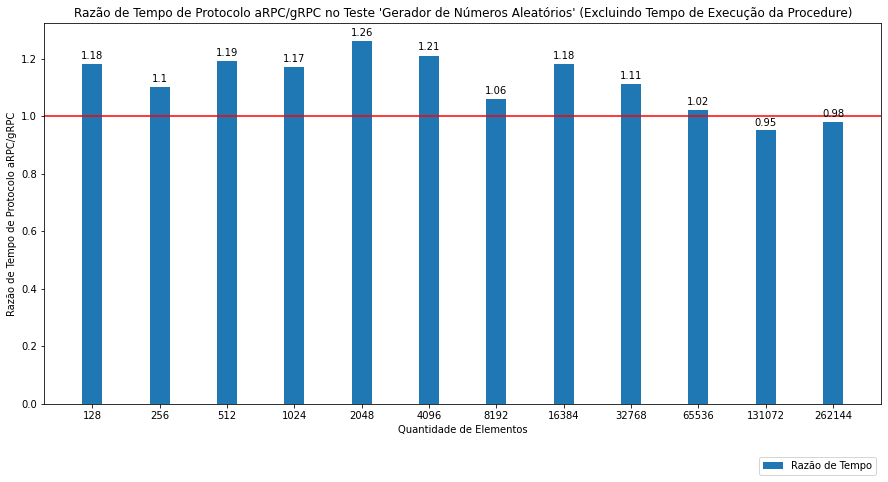
\includegraphics[width=\textwidth]{figuras/framework/razao_tempo_execucao_getrandomnumbers.png}
    \label{fig:razao_tempo_execucao_getrandomnumbers}
\end{figure}

\begin{figure}[ht]
    \centering
    \caption{Razão do Tempo de execução do aRPC e do gRPC para o caso de teste \textbf{Média}}
    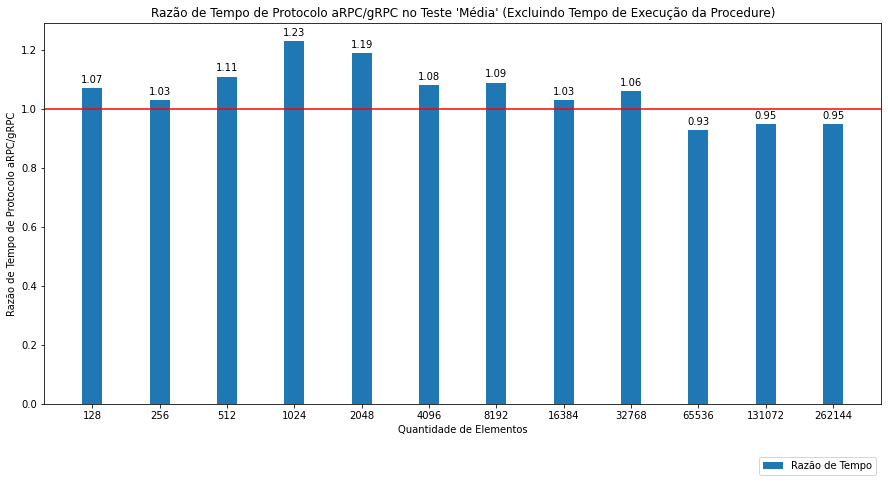
\includegraphics[width=\textwidth]{figuras/framework/razao_tempo_execucao_average.png}
    \label{fig:razao_tempo_execucao_average}
\end{figure}

Como pode ser visto nas Figuras \ref{fig:razao_tempo_execucao_largedata}, \ref{fig:razao_tempo_execucao_getrandomnumbers} e \ref{fig:razao_tempo_execucao_average}, respectivamente referentes aos testes \textbf{Ecoar}, \textbf{Gerador de Números Aleatórios} e \textbf{Média}, o aRPC possui um desempenho pior que a do gRPC para uma quantidade de elementos inferior a 65536. A partir desse valor o aRPC se iguala e então começa a ficar mais rápido que o gRPC com ganhos de 2\% a 7\%. A partir de uma quantidade grande suficiente de números, os ganhos de \textit{speedup} do serializador, somado as reduções de sobrecarga proporcionadas pelo QUIC fazem com que o \textit{framework} escale melhor que o gRPC. Os ganhos mencionados tendem a aumentar conforme a quantidade de elementos aumenta até que a banda da rede esteja inteiramente saturada.

%No caso da Figura \ref{fig:razao_tempo_execucao_alltypes}, referente ao teste \textbf{Todos os Tipos} que como apresentado anteriormente representa melhor o uso esperado do \textit{framework}, foi obtido um resultado favorável mesmo para quantidade pequena de elementos. Esse ganho mesmo em quantidades pequenas de elementos advém de uma serialização mais eficiente em quantidade de bytes pelo Colfer como pode ser visto na Figura \ref{fig:razao_tamanho_alltypes}, que neste caso consegue performar melhor que o Protobuffers.

\begin{figure}[ht]
    \centering
    \caption{Razão do Tempo de execução do aRPC e do gRPC para o caso de teste \textbf{Todos os Tipos}}
    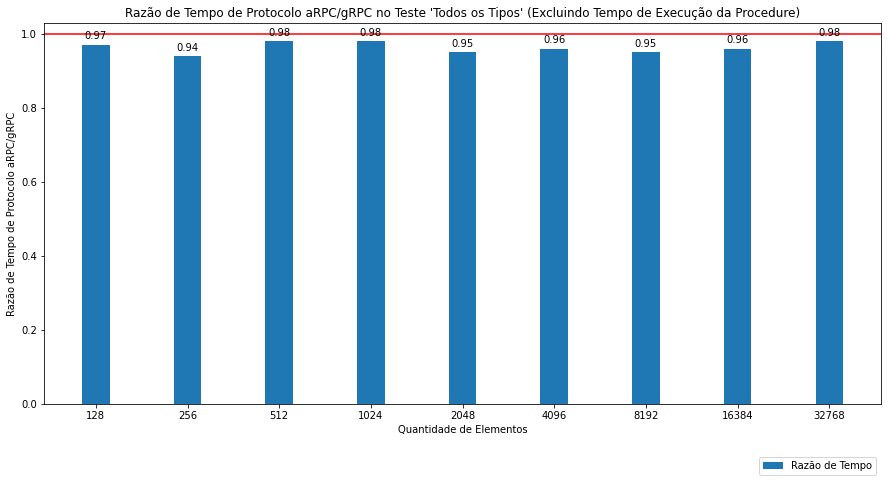
\includegraphics[width=\textwidth]{figuras/framework/razao_tempo_execucao_alltypes.png}
    \label{fig:razao_tempo_execucao_alltypes}
\end{figure}

A Figura \ref{fig:razao_tempo_execucao_alltypes} é referente ao teste \textbf{Todos os Tipos} que, como apresentado anteriormente, representa melhor o uso esperado do \textit{framework}. O resultado obtido foi favorável mesmo para uma quantidade pequena de elementos, sendo que o ganho nessas condições advém de uma serialização mais eficiente, em termos de quantidade de bytes, realizada pelo serializador Colfer em comparação com o serializador Protobuffers, conforme exemplificado na Figura \ref{fig:razao_tamanho_alltypes}.

A partir da análise dos dados coletados acima é possível concluir que, caso a serialização do Colfer seja mais eficiente ou igual ao Protobuffers, o aRPC pode ter um desempenho melhor ou igual ao gRPC. 

Já para grandes quantidades de elementos as vantagens do aRPC são mais evidentes e, nesses casos, mesmo em uma situação de serialização desvantajosa, o aRPC é mais eficiente, atingindo maior vazão.
